\begin{titlepage}

  \begin{figure}[H]
    \begin{center}
      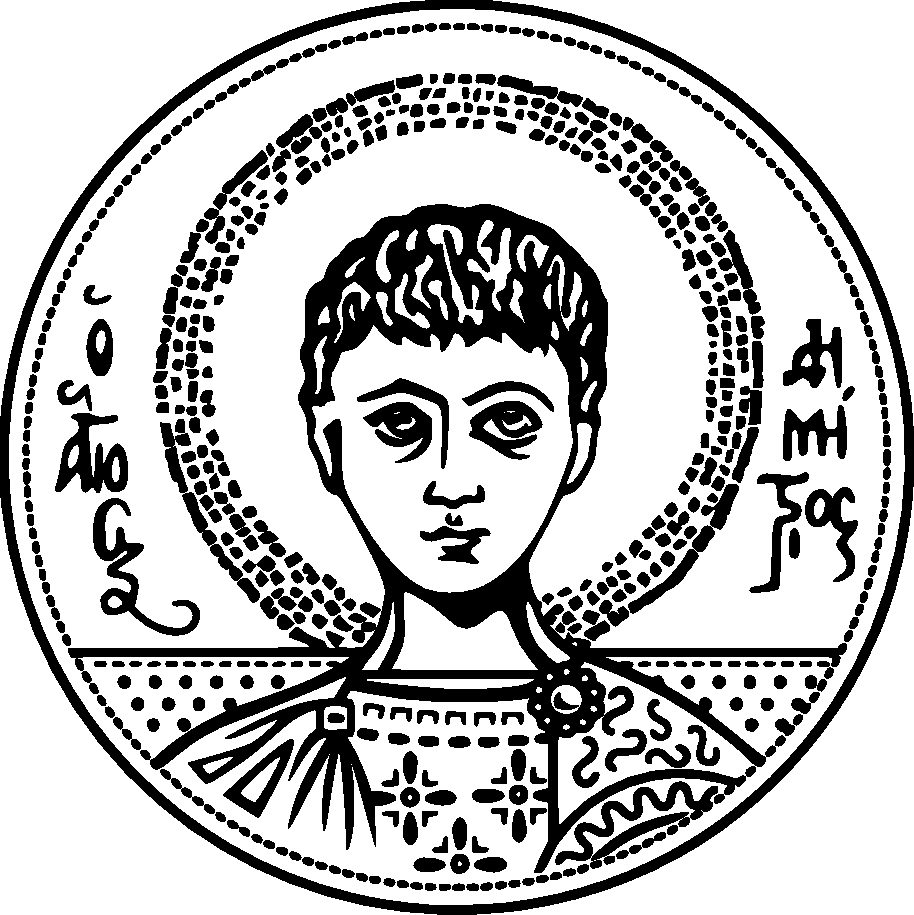
\includegraphics[width=3cm]{auth.pdf}
      \label{fig:cover_auth_logo}
    \end{center}
  \end{figure}

  \centering \Large Αριστοτέλειο Πανεπιστήμιο Θεσσαλονίκης\\ \Large
  Πολυτεχνική Σχολή\\ \large Τμήμα Ηλεκτρολόγων Μηχανικών και Μηχανικών
  Υπολογιστών\\ \large Τομέας Τηλεπικοινωνιών

  \vspace{
    \fill}

  \LARGE Τίτλος διπλωματικής

  \vspace{
    \fill}

  \Large Διπλωματική Εργασία\\ \Large του\\ \Large Θεοφάνη Θαρρόπουλου

  \vspace{
    \fill} \raggedright

  \begin{tabular}{ll}
    \textbf{Επιβλέπων:} & Ανδρέας Συμεωνίδης \\
    & Καθηγητής Α.Π.Θ.\\
  \end{tabular}

  \centering \vspace{
    \fill} \today

\end{titlepage}

\begin{abstract}
  Αντικείμενο της παρούσας διπλωματικής εργασίας αποτελεί η έρευνα για
  την αξιολόγηση της ποιότητας του κώδικα που παράγεται από Μεγάλα
  Γλωσσικά Μοντέλα \tl{(LLMs)}, και πιο συγκεκριμένα από το
  \textlatin{GitHub Copilot}\cite{githubcopilot}. Η μελέτη εστιάζει στην
  αξιολόγηση της ποιότητας του κώδικα που παράγεται από το Copilot και
  στην βελτιστοποίηση των προτροπών \textlatin{(prompts)} για την
  επίτευξη των επιθυμητών αποτελεσμάτων μέσω τεχνικών μηχανικής
  προτροπής \textlatin{(prompt engineering)} και της μηχανικής μάθησης.
  Τα αποτελέσματα αποδεικνύουν τις δυνατότητες και τους περιορισμούς του
  Copilot στην παραγωγή ποιοτικού κώδικα και προσφέρουν νέες
  προσεγγίσεις για την βελτίωση της αλληλεπίδρασης μεταξύ του χρήστη και
  του εργαλείου μέσω στοχευμένων τεχνικών προτροπής.
\end{abstract}

\selectlanguage{english}
\begin{abstract}
  Empty
\end{abstract}

\thispagestyle{empty}

\selectlanguage{greek}

\section*{Ευχαριστίες} \thispagestyle{empty}

Θα ήθελα να ευχαριστήσω τον επιβλέποντα της διπλωματικής εργασίας μου,
κ. Ανδρέα Συμεωνίδη, για την ευκαιρία που μου έδωσε να εργαστώ πάνω σε
ένα θέμα που με ενθουσιάζει και για την υποστήριξη που μου προσέφερε
καθ' όλη την διάρκεια της εργασίας μου, καθώς και για τη βοήθεια σε όσες
δυσκολίες βίωσα κατά την έρευνα. Επίσης, θα ήθελα να ευχαριστήσω τους
αγαπημένους μου φίλους, Θοδωρή, Παρασκευά, Λεωνίδα, Βασίλη, Ιορδάνη,
Λευτέρη, Θεοδόση, για την υπομονή και στήριξη που έδιξαν όλο αυτό τον
καιρό. θα ήθελα να ευχαριστήσω την αγαπημένη μου μητέρα, Βασιλική, για
τις θυσίες της όλα αυτά τα χρόνια, την αγάπη και δύναμη που μου έχει
δώσει από τη μέρα που γεννήθηκα, τον αγαπημένο μου πατέρα Χρήστο, που με
γέμιζε πάντοτε χαρά με την περιφάνεια του για μένα.

Τέλος, θα ήθελα να ευχαριστήσω περισσότερο από όλους, τον μοναδικό μου
αδερφό Γιώργο, το άτομο που αγαπώ και θαυμάζω περισσότερο από καθέναν
άλλον στον κόσμο. Τον πιο δυνατό, έξυπνο και αξιόλογο άνθρωπο που
γνώρισα ποτέ, που με παρότρυνε να σπουδάσω στο τμήμα των Ηλεκτρολόγων
Μηχανικών και Μηχανικών Υπολογιστών, που μου έμαθε να αγαπώ το έργο του
μηχανικού και τον προγραμματισμό και μου έδειξε πώς να παλεύω για ό,τι
αγαπώ. Χωρίς αυτόν η ζωή μου δεν θα ήταν απλώς φτωχότερη, μα άδεια. Από
την πρώτη μέρα στο πανεπιστήμιο, μέχρι και την τελευταία, ήταν το
στήριγμα, η συμβουλή, η κριτική, η αγάπη και η φιλία που με κράτησαν
όρθιο και με έκαναν να πιστεύω στον εαυτό μου. Ελπίζω να είμαι έστω και
στο ελάχιστο τόσο καλός όσο είναι αυτός, και να τον κάνω περήφανο, όπως
πάντοτε με έκανε ο ίδιος.
